\documentclass[10pt]{article}
\usepackage[margin=0.72in]{geometry}
\usepackage[T1]{fontenc}
\usepackage{graphicx}
\usepackage{amsmath}
\usepackage{amssymb}
\usepackage{array}
\setlength{\parskip}{0.45em}
\setlength{\parindent}{0pt}
\begin{document}
\begin{center}
{\Large\bfseries NCP commutator-ideal refutation}\par
{\small 2026-10-21; THM-COMMUTATOR-KERNEL1 Proposition 1; TASK-20260822-b69d29}
\end{center}

\textbf{Scope.} The free associative $\mathbb Z$-algebra $A$ has generators
$t_1,\ldots,t_B,v$. Let $I$ be the two-sided ideal generated by all
commutators $xy-yx$. Evaluation $\rho$ sends $t_i$ to translation by $s_i$
and $v$ to negation in the group algebra of the affine permutation group of
$\mathbb Z/n\mathbb Z$. The Lean theorem proves $\ker\rho\ne I$ for every
$B,n$, and translation list $s$.

\section*{Witness and separation}
Set $w=v^2-1$. Negation is an involution even when $n=1$ or $2$, so
$\rho(w)=0$. The algebra homomorphism $\varepsilon:A\to\mathbb Z$ sending
every free generator to zero kills all commutators, hence $I\subseteq
\ker\varepsilon$. But $\varepsilon(w)=-1\ne0$. Therefore $w\notin I$ and
$\ker\rho\ne I$. This argument separates the witness without constructing
the whole commutative-polynomial quotient.

\begin{center}
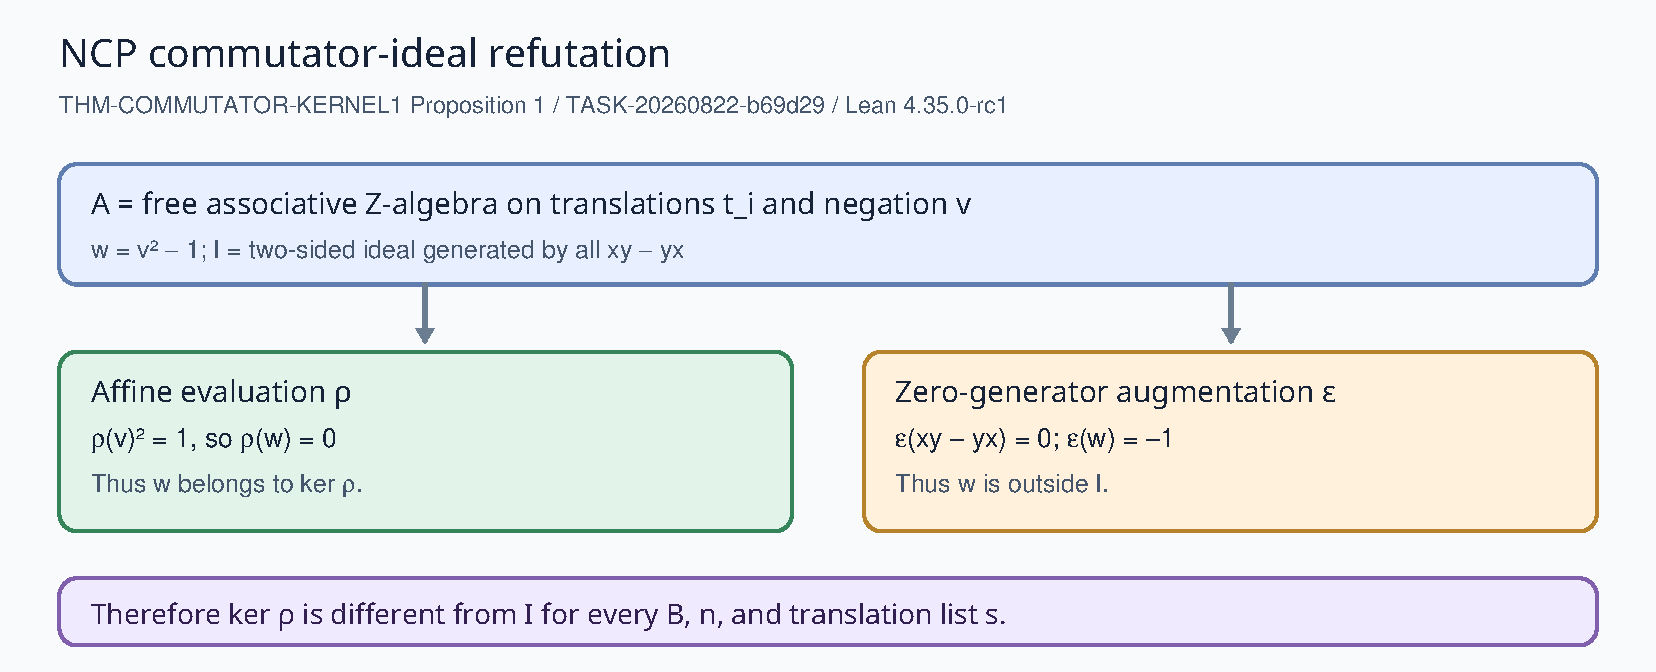
\includegraphics[width=\linewidth]{diagram.pdf}
\end{center}

\section*{Validation and limits}
\begin{tabular}{|p{0.31\linewidth}|p{0.59\linewidth}|}\hline
Check & Observed result \\ \hline
Pinned Lean target & Machine verified on Lean 4.35.0-rc1; 2,077 build jobs passed; project audit passed 506 theorem declarations using standard axioms only. \\ \hline
Named theorem axioms & \texttt{propext}, \texttt{Classical.choice}, and \texttt{Quot.sound}; no \texttt{sorry} or extra axioms. \\ \hline
Complete target corpus & 66 machine verified; zero failed, zero infrastructure failures, zero undischarged. All 66 receipts bind to the source commit; all require independent semantic review. \\ \hline
\end{tabular}

The proof is uniform; it therefore covers instances where the given list
makes evaluation surjective. It does not itself establish surjectivity for
arbitrary lists, the full kernel presentation, or algorithmic performance.
Independent semantic review remains pending. No timing datum was produced,
so canonical numerical dashboards are unchanged.

\end{document}
